\chapter{Introducción}

La mecánica cuántica es la teoría en Física que describe el comportamiento de la materia a escala atómica y subatómica (Feynman, Leighton y Sands, 1964). Su orígen suele ubicarse en dos artículos: uno de Max Planck (1901) que resolvía el problema conocido como la Catástrofe Ultravioleta proponiendo una discretización de la energía y otro Albert Einstein (1905) que daba una explicación satisfactoria para el efecto fotoeléctrico suponiendo que la luz se presentaba en forma de partículas. A lo largo del siglo XX, un gran número de científicos contribuyeron al desarrollo de esta disciplina introduciendo importantes conceptos tales como el principio onda-corpúsculo (De Broglie, 1924), la ecuación de Schrödinger (1926) o el principio de incertidumbre (Heisenberg, 1927), entre otros. 

A principios de los 80, Richard Feynman (1982) señaló que existían ciertos problemas físicos cuya simulación requería recursos que crecían de manera exponencial. La observación de esta dificultad ponía de manifiesto la necesidad de un nuevo paradigma de computación basado en los efectos de la mecánica cuántica. De esta manera, nace la computación cuántica.

En este contexto, el bit clásico encuentra su contrapartida cuántica, el qubit (Schumacher, 1995). Así pues, los estados con lo que se puede computar dejan de ser únicamente los estados “0” y “1” si no también cualquier posible superposición cuántica de dichos estados. No obstante, es sabido que los estados cuánticos son efímeros y volátiles y tienen tendencia a destruirse, fenómeno conocido como pérdida de la coherencia cuántica (o decoherencia cuántica). Por lo tanto, uno de los requisitos que debe cumplir un qubit es que la capacidad de mantener su coherencia cuántica durante el tiempo suficiente para que pueda operarse sobre él (Divincenzo, 2000)


La dificultad para mantener la coherencia en sistemas cuánticos ha sido siempre un gran obstáculo en el desarrollo de la computación cuántica. Por este motivo, la corrección cuántica de errores ha sido siempre un campo de gran interés en el ámbito del procesamiento de información cuántica (Devitt, Munro y Nemoto, 2013). 

En este sentido, la publicación del código de Shor (1995) fue un avance de gran interés ya que fue el primer algoritmo de corrección cuántica de errores funcional y abrió la puerta para superar el obstáculo frente al que se encontraba el desarrollo de la computación cuántica. Se trata de un código degenerado que permite la corrección de un error de amplitud y un error de fase en un qubit.

No obstante, mientras que la implementación del código propiamente dicho se encuentra bien documentada en fuentes tales como Quantum Computation and Quantum Information (Nielsen y Chuang, 2001) o el artículo original de Shor (1995), no se han encontrado implementaciones específicas del circuito correspondiente al cálculo del síndrome. Así pues, este trabajo pretende rellenar este vacío aportando posibles implementaciones de dicho circuito contempladas desde diferentes prismas. 

Las distintas versiones de dicho circuito que se propondrán en este proyecto atienden, principalmente, a dos líneas de trabajo: en una de ellas, se hará uso de los recursos del computador sin restricción y, en la otra, se priorizará minimizar el número de qubits a costa de reutilizar los mismo con el consiguiente gasto energético. 



\textbf{Duda: Supongo que esto también implicará un mayor tiempo de ejecución (al menos así suele ser en computación clásica}

















---------------------------------------------

El primer capítulo es siempre una introducción. En ella debes resumir de forma esquemática pero suficientemente clara lo esencial de cada una de las partes del trabajo. La lectura de este primer capítulo ha de dar una primera idea clara de lo que se pretendía, las conclusiones a las que se ha llegado y del procedimiento seguido.

Como tal, es uno de los capítulos más importantes de la memoria. Las ideas principales a transmitir son la identificación del problema a tratar, la justificación de su importancia, los objetivos generales (a grandes rasgos) y un adelanto de la contribución que esperas hacer.

Típicamente una introducción tiene tres apartados: Motivación, Planteamiento del trabajo, Estructura del trabajo. (Texto Normal del menú de estilos.)

(Ejemplo de nota al pie\footnote{Ejemplo de nota al pie.}.)

\section{Motivación/justificación del tema a tratar}

¿Cuál es el problema que quieres tratar?

¿Cuáles crees que son las causas?

¿Por qué es relevante el problema?

A continuación, se indica con un ejemplo cómo deben introducirse los títulos y las fuentes en Tablas y Figuras.

\begin{table}[t]
	\begin{center}
	\caption{Ejemplo de tabla con sus principales elementos.}
	\label{tab:tab-1}
	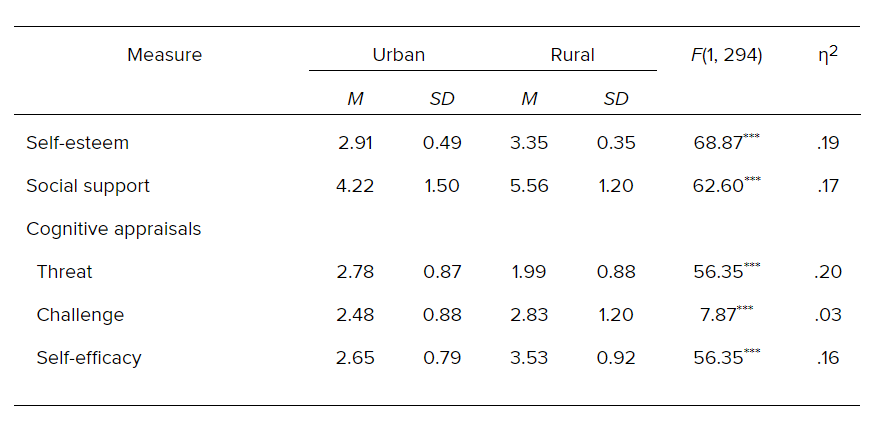
\includegraphics[width=4.90737in,height=2.42708in]{tabla}

	\small Fuente: American Psychological Association, 2020e.
	\end{center}
\end{table}

\begin{figure}[ht]
	\begin{center}
		\caption{Ejemplo de figura realizada para nuestro trabajo.}
		\label{fig:fig-1}
		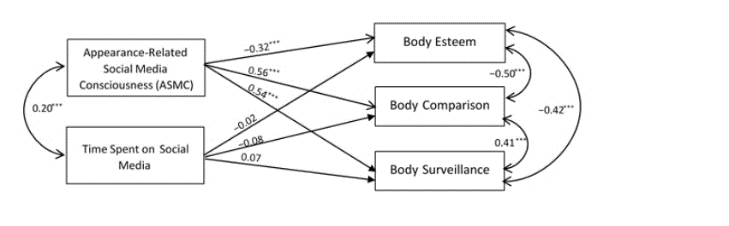
\includegraphics[width=4.90737in,height=2.42708in]{figura}

		\small Fuente: American Psychological Association, 2020f.
	\end{center}
\end{figure}

\section{Planteamiento del trabajo/problema}

¿Cómo se podría solucionar el problema?

¿Qué es lo que se propone?

Aquí describes tu objetivo en términos generales.

\section{Estructura del trabajo}

Aquí describes brevemente lo que vas a contar en cada uno de los capítulos siguientes.